\documentclass[11pt]{scrartcl}
\usepackage{tikz,tkz-tab,amsmath}
\usepackage{polski}
\usepackage[miktex]{gnuplottex}
\usepackage[T1]{fontenc}
\usepackage[utf8]{inputenc}
\usetikzlibrary{arrows}
\usepackage{amssymb}
\usepackage{graphicx}
\graphicspath{ {images/} }
\title{Przebieg zmienności funkcji}
\author{Jakub Hajto}

\everymath{\displaystyle}
\begin{document}
	\maketitle
	\begin{center}
	Badana funckja $$ f(x) = \frac{x(x+1)}{x-1} $$
	\end{center}
	\begin{enumerate}  
		\item Dziedzina: \\
			$ D = \mathbb{R} \backslash \{1\} $
		\item Zbiór wartości: \\
			$ Z_w = (-\infty, 3 - 2\sqrt{2}) \cup (3 + 2\sqrt{2}, + \infty) $
		\item Miejsca zerowe: \\
			$ f(x) = 0 \Longleftrightarrow x = -1 \vee x = 0 $
		\item Przecięcie z osią OY: \\
			f(0) = 0
		\item Granice na krańcach przedziałów:
			\begin{enumerate}
				\item $ \lim_{x\to\infty} f(x) = -\infty $
				\item $ \lim_{x\to1^-} f(x) = -\infty $
				\item $ \lim_{x\to1^-} f(x) = +\infty $
				\item $ \lim_{x\to+\infty} f(x) = +\infty $
			\end{enumerate}
		\item Asymptoty:
			\begin{enumerate}
				\item ukośna: \\
					$ y = x + 2$
				\item pionowa: \\
					$ x=1 $
			\end{enumerate}
		\item Pierwsza pochodna \\
			$ f^{\prime}(x) = \frac{x^2 - -2x -1}{(x-1)^2} =  \frac{(x- \sqrt{2} - 1)(x + \sqrt{2} - 1)}{(x-1)^2} $
			\begin{enumerate}
				\item $ f\nearrow dla x \in (-\infty, \sqrt{2} -1) \cup (\sqrt{2} +1, +\infty) $
				\item $ f\searrow x \in ( \sqrt{2} - 1, \sqrt{2} +1 ) $
				\item Ekstrema lokalne:
					\begin{enumerate}
						\item W $ x = \sqrt{2} -1 $ istnieje maximum lokalne równe $ 3 - 2\sqrt{2} $
						\item W $ x = \sqrt{2} + 1 $ istnieje maximum lokalne równe $ 3+ 2\sqrt{2} $
					\end{enumerate}
			\end{enumerate}
		\item Druga pochodna \\
			$ f^{\prime\prime}(x) = \frac{4}{(x-1)^3} $
			\begin{enumerate}
				\item Przedziały wypukłości ku górze \\
				$ f\cap \Leftrightarrow x \in (-\infty, 1) $
				\item Przedziały wypukłości ku dołowi \\
				$ f\cup \Leftrightarrow x \in (1,\infty) $
			\end{enumerate}
		\item Tabela \\
			\begin{center}
				\begin{tabular}{ |c|c|c|c|c| } 
					\hline
					Przedziały &
						$ (-\infty, \sqrt{2} -1) $ &
						$ \sqrt{2} -1 $ & 
						$ (\sqrt{2} -1, 1) $ &
						$ 1 $ \\
					$ f(x) $ &
						$ -\infty \to 3 - 2\sqrt{2} $ &
						$ Max 3 - 2\sqrt{2} $ &
						$ (3 - 2\sqrt{2}, -\infty) $ &
						$ \times $ \\
					$ f^{\prime}(x) $ &
						+ &
						0 &
						- &
						$ \times $ \\
					\hline
				\end{tabular}
				\begin{tabular}{ |c|c|c|c| } 
				\hline
				Przedziały &
					$ (1, \sqrt{2} + 1) $ &
					$ \sqrt{2} + 1 $ &
					$ (\sqrt{2} + 1, +\infty) $\\
				$ f(x) $ &
					$ \infty \to 3 + 2\sqrt{2} $ &
					$ 3 + 2\sqrt{2} $ &
					$ (3 + 2\sqrt{2}, + \infty) $ \\
				$ f^{\prime}(x) $ &
					- &
					0 &
					+  \\
				\hline
				\end{tabular}
			\end{center}
		\item Wykres funkcji \\
			\begin{center}
				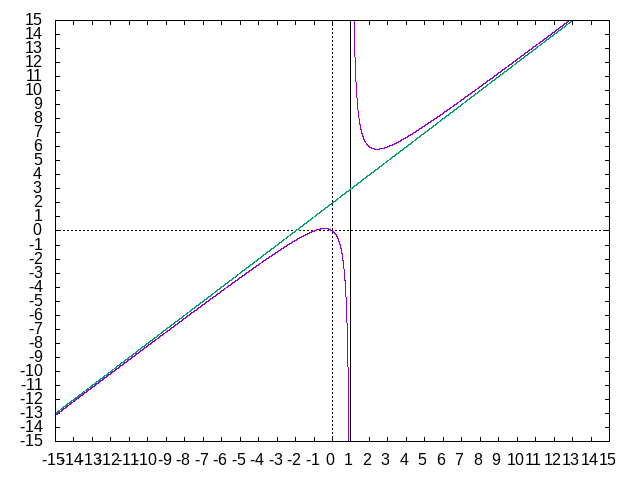
\includegraphics[scale=0.6]{funkcja1}
			\end{center}
			
	\end{enumerate}

	
\end{document}